% SPDX-FileCopyrightText: Copyright (c) 2023-2025 Yegor Bugayenko
% SPDX-License-Identifier: MIT

\documentclass{article}
\usepackage{../lecture-notes/notes}
\newcommand*\thetitle{Algorithms}
\newcommand*\thesubtitle{History, State, Behavior, Enemies of OOP}
\begin{document}

\lnTitlePage{1}{8}{8FPU_N3LxqA}

\pptToc

\lnPitch{
    \pptBanner[red]{WARNING!}
    In the pursuit of academic enlightenment within this course, it is paramount to caution that the doctrines disseminated may present a potentially \ul{hazardous venture} if employed in real-life software projects. This inherent risk arises from the potential \ul{incongruity} with the broadly accepted \ul{canon} of object-oriented programming and recognized best programming practices. If one remains resolute in their decision to adapt their coding methodologies to align with the principles propagated in this course, it would be prudent to employ a certain degree of \ul{foresight}. A humorous, yet sincere suggestion, would be to secure \ul{alternate employment} prior to a possible premature termination of one's current professional engagement.}

\lnPitch{\pptChapter{Pre-Test}}

\begin{lnSnippet}[java-parser.txt]
public class Parser {
  private File file;
  public synchronized void setFile(File f) {
    file = f;
  }
  public synchronized File getFile() {
    return file;
  }
  public String getContent() throws IOException {
    // Read the content of the file
    // and return it.
  }
  public String getContentWithoutUnicode() throws IOException {
    // Read the file and filter out symbols
    // that are not UTF-8 compliant.
  }
  public void saveContent(String content) {
    // Save the "content" to the file.
  }
}
\end{lnSnippet}
\lnPitch{
  \pptSection[quiz]{https://github.com/yegor256/quiz}
  {\scriptsize\ffinput{java-parser.txt}}}

\lnPitch{\pptChapter{History}}

\lnPitch{
    \pptSection[Sketchpad]{Who Started It?}
    \pptPic{0.5}{ivan-sutherland-with-computer.jpg}\\
    Ivan Sutherland's seminal \textbf{Sketchpad} \ul{application} was an early inspiration for OOP, created between 1961 and 1962 and published in his Sketchpad Thesis in 1963. Any object could become a ``master,'' and additional instances of the objects were called “occurrences”. Sketchpad's masters share a lot in common with JavaScript's prototypal inheritance. \textcolor{gray}{(c)~Wikipedia}
}

\lnPitch{
    \pptSection[Objects]{Who Invented Objects, Classes, and Inheritance?}
    \pptPic{0.6}{dahl-and-nygaard.jpg}\\
    \textbf{Simula} was developed in 1965 at the Norwegian Computing Center in Oslo, by Ole-Johan Dahl and Kristen Nygaard. Like Sketchpad, Simula featured objects, and eventually introduced \ul{classes}, class \ul{inheritance}, \ul{subclasses}, and \ul{virtual methods}. \textcolor{gray}{(c)~Wikipedia}
}

\begin{lnSnippet}[simula.txt]
Class Figure;
  Virtual: Real Procedure area Is Procedure area;;
Begin
End;
Figure Class Circle (c, r);
  Real c, r;
Begin
  Real Procedure area;
  Begin
    area := 3.1415 * r * r;
  End;
End;
\end{lnSnippet}
\lnPitch{
  \pptSection[Simula-67]{Simula-67: Sample Code}
  \ffinput{simula.txt}}

\lnPitch{
    \pptSection[OOP]{Who Coined the ``OOP'' Term?}
    \pptPic{0.6}{smalltalk-guys.jpg}\\
    \textbf{Smalltalk} was created in the 1970s at Xerox PARC by Learning Research Group (LRG) scientists, including
    Alan Kay, Dan Ingalls, Adele Goldberg, Ted Kaehler, Diana Merry, and Scott Wallace. \textcolor{gray}{(c)~Wikipedia}}

\begin{lnSnippet}[smalltalk.txt]
Object subclass: Account [
    (*@\(\vert\)@*) balance (*@\(\vert\)@*)
    Account class >> new [
        (*@\(\vert\)@*) r (*@\(\vert\)@*)
        r := super new. r init. ^r
    ]
    init [ balance := 0 ]
]
Account extend [
    deposit: amount [ balance := balance + amount ]
]
a := Account new
a deposit: 42
\end{lnSnippet}
\lnPitch{
  \pptSection[Smalltalk]{Smalltalk: Sample Code}
  {\small\ffinput{smalltalk.txt}}}

\lnQuote
  {professor}
  {Everyone will be in a favor of OOP. Every manufacturer will promote his products as supporting it. Every manager will pay lip service to it. Every programmer will practice it (differently). And no one will know just what it is.}
  {rentsch1982object}

\lnPitch{
    \pptSection[Stroustrup]{Who Made It All Popular?}
    \pptPic{0.7}{bjarne-in-1985.jpg}\\
    \textbf{C++} was created by Danish computer scientist Bjarne Stroustrup in 1985, by enhancing the C language with Simula-like features. C was chosen because it was general-purpose, fast, portable and widely used.\par
    {\small You may enjoy watching this \href{https://www.youtube.com/watch?v=ae6nFZn3auQ}{one-hour dialog} of Dr. Stroustrup and me.}}

\begin{lnSnippet}[cpp.txt]
class Figure {
  virtual float area() = 0;
};
class Circle : public Figure {
  Circle(float c, float r) : c(c), r(r) {};
  float area() { return 3.1415 * r * r; };
private:
  float c, r;
};
\end{lnSnippet}
\lnPitch{
  \pptSection[C++]{C++: Sample Code}
  \ffinput{cpp.txt}}

\lnQuote
  [Ole Lehrmann Madsen]
  {ole-lehrmann-madsen}
  {There are as many definitions of OOP as there are papers and books on the topic.}
  {madsen1988object}

\lnQuote
  {alan-kay}
  {I made up the term `object-oriented,' and I can tell you I didn't have C++ in mind.}
  {kay97keynote}

\lnPitch{
  There was an interesting debate between Alan Kay and a few readers of my blog, in the comments section under this blog post:
  \href{https://www.yegor256.com/2017/12/12/alan-kay-was-wrong.html}{Alan Kay Was Wrong About Him Being Wrong}~\citep{bugayenko2017blog1212}.}

\lnPitch{
  \pptSection[Languages]{What Happened Later?}
  C++ was released in 1985. And then...\par
  \begin{multicols}{2}
  Erlang (1986) \\
  Eiffel (1986) \\
  Self (1987) \\
  Perl (1988) \\
  Haskell (1990) \\
  Python (1991) \\
  Lua (1993) \\
  JavaScript (1995) \\
  Ruby (1995) \\
  Java (1995) \\
  PHP3 (1998) \\
  C\# (2000) \\
  Go (2009) \\
  Rust (2010) \\
  Swift (2014) \\
  \href{https://www.eolang.org}{EO} (2016)
  \end{multicols}}

\lnQuote
  {oscar-nierstrasz}
  {There is no uniformity or an agreement on the set of features and mechanisms that belong in an OO language as the paradigm itself is far too general.}
  {nierstrasz1989survey}

\lnPitch{
  \pptSection[Features]{Incomplete List of OOP Features, ... So Far:}
  {\small\begin{pptWide}{4}
  Polymorphism \\
  Nested Objects \\
  Traits \\
  Templates \\
  Generics \\
  Invariants \\
  Classes \\
  NULL \\
  Exceptions \\
  Operators \\
  Methods \\
  Static Blocks \\
  Virtual Tables \\
  Coroutines \\
  Monads \\
  Algebraic Types \\
  Annotations \\
  Interfaces \\
  Constructors \\
  Destructors \\
  Lifetimes \\
  Volatile Variables \\
  Synchronization \\
  Macros \\
  Inheritance \\
  Overloading \\
  Tuple Types \\
  Closures \\
  Access Modifiers \\
  Pattern Matching \\
  Enumerated Types \\
  Namespaces \\
  Modules \\
  Type Aliases \\
  Decorators \\
  Lambda Functions \\
  Type Inference \\
  Properties \\
  Value Types \\
  Multiple Inheritance \\
  Events \\
  Callbacks \\
  NULL Safety \\
  Streams \\
  Buffers \\
  Iterators \\
  Generators \\
  Aspects \\
  Anonymous Objects \\
  Anonymous Functions \\
  Reflection \\
  Type Casting \\
  Lazy Evaluation \\
  Garbage Collection \\
  Immutability
  \end{pptWide}}}

\lnQuote
  [Edsger Dijkstra]
  {edsger-dijkstra}
  {Object oriented programs are offered as alternatives to correct ones... Object-oriented programming is an \ul{exceptionally bad idea} which could only have originated in California.}
  {crawford1989}

\lnQuote
  [Alan Kay]
  {alan-kay}
  {I made up the term `object-oriented,' and I can tell you I didn't have C++ in mind.}
  {kay97keynote}

\lnQuote
  [Linus Torvalds]
  {linus-torvalds}
  {C++ is a \ul{horrible language}$\dots$ C++ leads to really, really bad design choices$\dots$ In other words, the only way to do good, efficient, and system-level and portable C++ ends up to limit yourself to all the things that are basically available in C.}
  {schindler2007}

\lnQuote
  [Jeff Atwood]
  {jeff-atwood}
  {OO seems to bring at least as \ul{many problems} to the table as it solves.}
  {atwood2007}

\lnQuote
  [Rich Hickey]
  {rich-hickey}
  {I think that large objected-oriented programs struggle with increasing complexity as you build this large object graph of \ul{mutable objects}. You know, trying to understand and keep in your mind what will happen when you call a method and what will the side effects be.}
  {hickey2010}

\lnPitch{\pptThought{The \ul{complexity} of object-oriented code remains its primary drawback}}

\lnQuote
  {asaf-shelly}
  {Reading an OO code you can't see the big picture and it is often impossible to review all the small functions that call the one function that you modified.}
  {shelly2015flaws}

\lnPitch{
  \pptThought{Thus, we don't know anymore what exactly is object-oriented programming, and whether it helps us write better code.}
  \par
  {\small You can find more quotes in this blog post of mine: \href{https://www.yegor256.com/2016/08/15/what-is-wrong-object-oriented-programming.html}{What's Wrong With Object-Oriented Programming?}~\citep{bugayenko2016blog0815}}\par}

\lnPitch{\pptChapter[Intent]{Original Intent}}

\lnQuote
  {david-parnas}
  {It is almost always incorrect to begin the decomposition of a system into modules on the basis of a flowchart. We propose instead that one begins with a list of \ul{difficult} design decisions or design decisions which are \ul{likely to change}. Each module is then designed to \ul{hide} such a decision from the others.}
  {parnas1972criteria}

\lnQuote
  {david-west}
  {The contemporary mainstream understanding of objects (which is not behavioral) is but a pale shadow of the original idea and antithetical to the original intent.}
  {west2004object}

\lnPitch{You may enjoy watching our conversation with Dr. David West, video-recorded and published on YouTube:
  \href{https://www.youtube.com/watch?v=s-hdZZzMCac}{part I}
  and
  \href{https://www.youtube.com/watch?v=bW5K5cJ-AVs}{part II}.}

\lnPitch{
  \pptThought{A system is a composition of objects that are abstractions, which hide data and expose behavior*}
  \par
  {\small * This is how I understand the original intent.}}

\begin{lnSnippet}[file-js.txt]
var file = {
  path: '/tmp/data.txt',
  read: function() { ... },
  write: function(txt) { ... }
}
\end{lnSnippet}
\lnPitch{
  \pptSection[Abstraction]{1) What Is an ``Abstraction''?}
  \begin{pptWide}{2}
  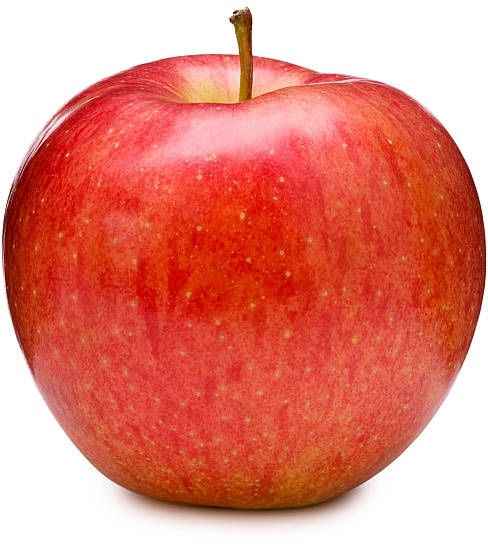
\includegraphics[width=1.3in]{apple.jpg}
  \begin{itemize}
  \item Color: red
  \item Weight: 120g
  \item Price: \$0.99
  \end{itemize}
  \par\columnbreak\par
  
\includegraphics[width=0.8in]{file-on-disc.jpg}
  \par
  {\small\ffinput{file-js.txt}}
  \end{pptWide}
  We deal with an abstraction as if it was a real thing, but eliminating unnecessary details.
  We do \ff{file.read()} instead of ``open file handler for data.txt, read byte by byte, store in
  byte buffer, wait for the end of file, and return the result.''}

\lnPitch{
  \begin{multicols}{2}
  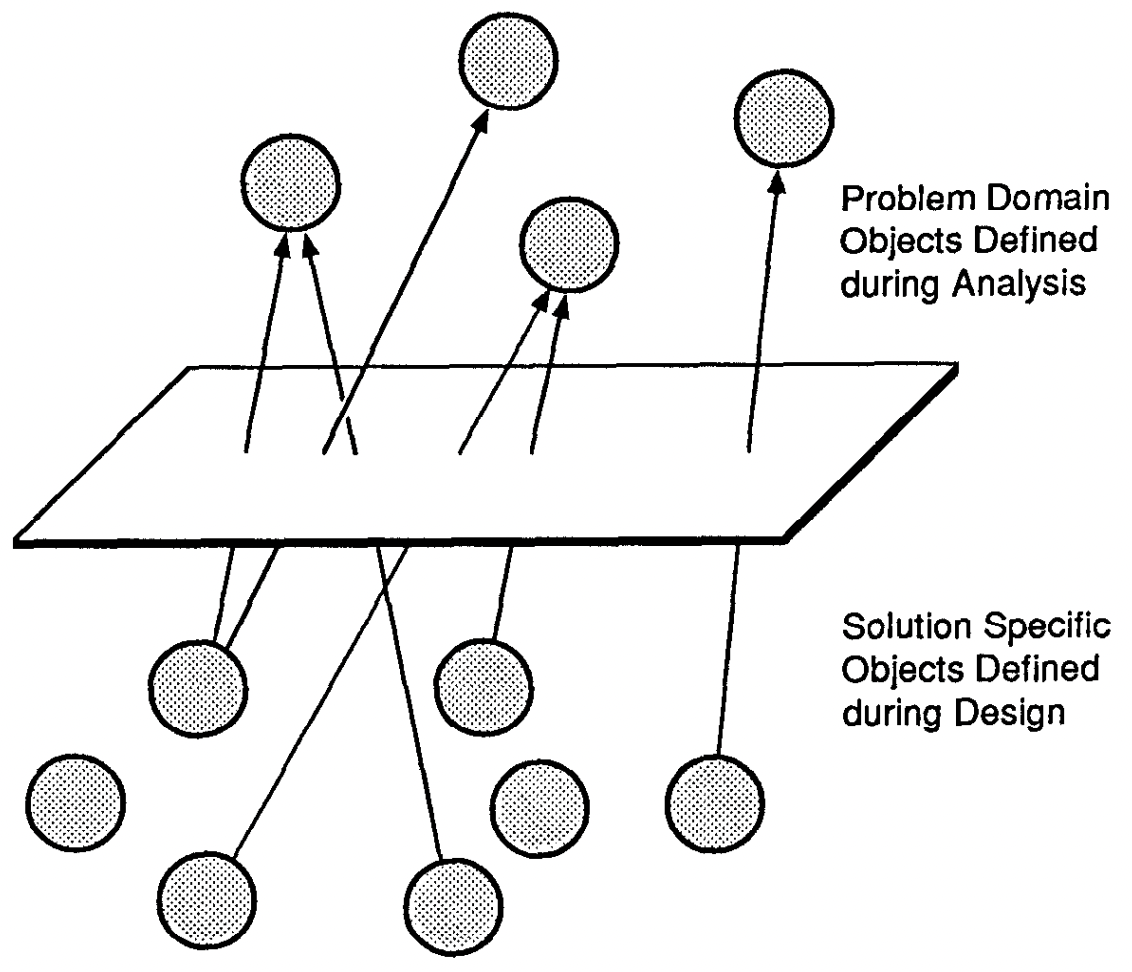
\includegraphics[width=.95\linewidth]{abstraction.png}
  \par\columnbreak\par
  ``Object-oriented design is first concerned with entities---things. These things may be tangible objects such as traffic lights, chairs, or airplanes. The entities may be abstract concepts such as roles, interactions, or incidents. From a design perspective, objects model the entities in the application domain.''
  \lnSource{korson1990understanding}
  \end{multicols}}

\lnQuote
  {edsger-dijkstra}
  {The effective exploitation of his \ul{powers of abstraction} must be regarded as one of the most vital activities of a competent programmer... By suitable application of our powers of abstraction, the intellectual effort required to conceive or to understand a program need not grow more than proportional to program length.}
  {dijkstra1972humble}

\begin{lnSnippet}[area-1.txt]
int area(x1, y1, x2, y2) {
  int w = x2 - x1;
  if (w < 0) { w = w * -1; }
  int h = y2 - y1;
  if (h < 0) { h = h * -1; }
  return w * h;
}
\end{lnSnippet}
\begin{lnSnippet}[area-2.txt]
int distance(left, right) {
  int d = right - left;
  if (d < 0) { d = d * -1; }
  return d;
}

int area(x1, y1, x2, y2) {
  return distance(x2, x1)
    * distance(y2, y1);
}
\end{lnSnippet}
\lnPitch{
  \pptSection[Rectangle]{How Many Abstractions Are Needed?}
  \begin{pptWide}{2}
  {\small\ffinput{area-1.txt}}
  \par\columnbreak\par
  {\small\ffinput{area-2.txt}}
  \end{pptWide}\par
  There are two abstractions at the right snippet (``area'' and ``distance''), while only one abstraction at the left one (just ``area'').}

\begin{lnSnippet}[distance.txt]
int distance(left, right) {
  int d = right - left;
  if (d < 0) { d = d * -1; }
  return d;
}

int area(x1, y1, x2, y2) {
  return distance(x2, x1)
    * distance(y2, y1);
}
\end{lnSnippet}
\lnPitch{
  \pptSection[Levels]{Levels of Abstraction}
  \begin{pptWide}{2}
  {\small\ffinput{distance.txt}}
  \par\columnbreak\par
  \begin{tikzpicture}[line width=2pt]
  \node[draw,rectangle,anchor=center] (area) {\texttt{area(3, 9, 13, 2)}};
  \node[draw,rectangle,below left=3cm and 0cm of area,anchor=center] (d1) {\texttt{distance(13, 3)}};
  \node[draw,rectangle,below right=3cm and 0cm of area,anchor=center] (d2) {\texttt{distance(2, 9)}};
  \draw[->] (area) -- (d1);
  \draw[->] (area) -- (d2);
  \end{tikzpicture}
  \end{pptWide}\par
  Higher level abstractions must not know and/or rely on semantics of lower level abstractions.}

\begin{lnSnippet}[hiding-1.txt]
f = new File("/tmp/data.txt");
// The data escapes the object! :(
p = f.getPath();
FileUtils.deleteFile(p);
\end{lnSnippet}
\begin{lnSnippet}[hiding-2.txt]
f = new File("/tmp/data.txt");
// The boolean data escapes too :)
done = f.delete();
assert(done);
\end{lnSnippet}
\lnPitch{
  \pptSection[Rectangle]{2) What Is ``Data Hiding''?}
  \begin{pptWide}{2}
  {\small\ffinput{hiding-1.txt}}
  \par\columnbreak\par
  {\small\ffinput{hiding-2.txt}}
  \end{pptWide}
  \par
  Obviously, some data must escape your objects.}

\begin{lnSnippet}[anemic.txt]
var user = {
  login: 'jeff',
  password: 'swordfish',
  age: 32
}
function print(u) {
  console.log(`Hello, ${u.login},
    you are ${u.age} today!`);
}
print(user);
\end{lnSnippet}
\begin{lnSnippet}[alive.txt]
var user = {
  login: 'jeff',
  password: 'swordfish',
  age: 32,
  print: function() {
    console.log(`Hello, ${this.login},
      you are ${this.age} today!`);
  }
}
user.print();
\end{lnSnippet}
\lnPitch{
  \pptSection[Rectangle]{3) What Is ``Behavior Exposing''?}
  \begin{pptWide}{2}
  This is so called ``anemic'' object:
  {\small\ffinput{anemic.txt}}
  \par\columnbreak\par
  This object is ``alive'':
  {\small\ffinput{alive.txt}}
  \end{pptWide}}

\begin{lnSnippet}[dist-1.txt]
int distance(left, right) {
  int d = right - left;
  if (d < 0) { d = d * -1; }
  return d; }
int area(x1, y1, x2, y2) {
  return distance(x2, x1)
    * distance(y2, y1); }
\end{lnSnippet}
\begin{lnSnippet}[dist-2.txt]
class Distance {
  private int r; private int l;
  Distance(a, b) { l = a; r = b; }
  int value() {
    int d = r - l;
    if (d < 0) { d = d * -1; }
    return d; } }
int area(x1, y1, x2, y2) {
  return new Distance(x2, x1).value()
    * new Distance(y2, y1).value(); } }
\end{lnSnippet}
\lnPitch{
  \pptSection[Function]{An Object as a Function}
  \begin{pptWide}{2}
  {\small\ffinput{dist-1.txt}}
  \par\columnbreak\par
  {\small\ffinput{dist-2.txt}}
  \end{pptWide}\par
  The Java object \ff{Distance} on the right snippet is semantically equivalent to the C function \ff{distance()} on the left one.}

\begin{lnSnippet}[identity-1.txt]
class Circle {
  private float radius;
  Circle(float r) {
    radius = r; }
  float getRadius() {
    return radius; }
  void setRadius(float r) {
    radius = r; }
  float area() {
    return 3.14 * radius * radius; }
}
\end{lnSnippet}
\begin{lnSnippet}[identity-2.txt]
// Identity:
c1 = new Circle(42.0);
c2 = new Circle(42.0);
c1 != c2;
// State:
c1 = new Circle(42.0);
c2 = new Circle(42.0);
c1.getRadius() == c2.getRadius();
// Behavior:
c1 = new Circle(42.0);
c2 = new Circle(-42.0);
c1.area() == c2.area();
\end{lnSnippet}
\lnPitch{
  \pptSection[State]{Identity, State, Behavior}
  \begin{pptWide}{2}
  {\small\ffinput{identity-1.txt}}
  \par\columnbreak\par
  {\small\ffinput{identity-2.txt}}
  \end{pptWide}}

\begin{lnSnippet}[state-1.txt]
class Circle {
  private float r;
  void setR(float r) { this.r = r; }
  float getR() { return this.r; }
}
class FigureUtils {
  static float area(Circle c) {
    return 3.14 * c.getR() * c.getR();
  }
}
Circle c = new Circle();
c.setR(42.0);
float s = FigureUtils.area(c);
\end{lnSnippet}
\begin{lnSnippet}[state-2.txt]
class Circle {
  private float r;
  Circle(float r) { this.r = r; }
  float area() {
    return 3.14 * this.r * this.r;
  }
}
Circle c = new Circle(42.0);
float s = c.area();
\end{lnSnippet}
\lnPitch{
  \pptSection[FigureUtils]{State vs. Behavior}
  \begin{pptWide}{2}
  {\small\ffinput{state-1.txt}}
  \par\columnbreak\par
  {\small\ffinput{state-2.txt}}
  \par
  How to decide what is \ul{state} and what is \ul{behavior}?
  \end{pptWide}}

\begin{lnSnippet}[composition-1.txt]
canvas = new Canvas();
canvas.addCircle(new Circle(42));
canvas.draw();
\end{lnSnippet}
\begin{lnSnippet}[composition-2.txt]
canvas = new Canvas();
circle = new Circle(42);
circle.drawOn(canvas);
\end{lnSnippet}
\lnPitch{
  \pptSection[Composition]{4) What Is ``Composition''?}
  \begin{pptWide}{2}
  {\small\ffinput{composition-1.txt}}
  \par\columnbreak\par
  {\small\ffinput{composition-2.txt}}
  \par
  \end{pptWide}
  What is composition? What is the ``right'' composition?}

\lnPitch{\pptChapter[O.T.]{Object Thinking vs. Algorithms}}

\begin{lnSnippet}[while-1.txt]
buffer = []
while true
  c = STDIN.readchar
  break if c == "\n"
  if buffer.length > 3
    STDOUT.puts buffer.join
    buffer = []
  end
  buffer << c
end
\end{lnSnippet}
\begin{lnSnippet}[while-2.txt]
$ echo 'Hello, world!' (*@\(\vert\)@*) ruby a.rb
Hell
o, w
orld
\end{lnSnippet}
\lnPitch{
  \pptSection[While]{While-Do Loop}
  \begin{pptWide}{2}
  {\small\ffinput{while-1.txt}}
  \par\columnbreak\par
  {\small\ffinput{while-2.txt}}
  \end{pptWide}}

\begin{lnSnippet}[buffer-1.txt]
buffer = []
while true
  c = STDIN.readchar
  break if c == "\n"
  if buffer.length > 3
    STDOUT.puts buffer.join
    buffer = []
  end
  buffer << c
end
\end{lnSnippet}
\begin{lnSnippet}[buffer-2.txt]
class Buffer
  def initialize; @data = []; end
  def push(c)
    if @data.length > 3
      STDOUT.puts @data.join
      @data = []
    end
    @data << c
  end
end
buffer = Buffer.new
while true
  c = STDIN.readchar
  break if c == "\n"
  buffer.push c
end
\end{lnSnippet}
\lnPitch{
  \pptSection[Buffer]{Buffer Abstraction}
  \begin{pptWide}{2}
  {\scriptsize\ffinput{buffer-1.txt}}
  \par\columnbreak\par
  {\scriptsize\ffinput{buffer-2.txt}}
  \end{pptWide}}

\begin{lnSnippet}[loop-1.txt]
class Buffer
  def initialize; @data = []; end
  def push(c)
    if @data.length > 3
      STDOUT.puts @data.join
      @data = []
    end
    @data << c
  end
end
buffer = Buffer.new
while true
  c = STDIN.readchar
  break if c == "\n"
  buffer.push c
end
\end{lnSnippet}
\begin{lnSnippet}[loop-2.txt]
class Buffer
  # the same
end
class Pull
  def initialize(b); @buf = b; end
  def again
    c = STDIN.readchar
    return false if c == "\n"
    @buf.push c
    true
  end
end
buffer = Buffer.new
pull = Pull.new(buffer)
while pull.again; end
\end{lnSnippet}
\lnPitch{
  \pptSection[Loop]{Loop Abstraction}
  \begin{pptWide}{2}
  {\scriptsize\ffinput{loop-1.txt}}
  \par\columnbreak\par
  {\scriptsize\ffinput{loop-2.txt}}
  \end{pptWide}}

\begin{lnSnippet}[loop-3.txt]
class Buffer
  # the same
end
class Pull
  def initialize(b); @buf = b; end
  def again
    c = STDIN.readchar
    return false if c == "\n"
    @buf.push c
    true
  end
end
buffer = Buffer.new
pull = Pull.new(buffer)
while pull.again; end
\end{lnSnippet}
\begin{lnSnippet}[loop-4.txt]
class Buffer
  # the same
end
class Pull
  # the same
end
class Pulls
  def initialize(p); @pull = p; end
  def fetch
    while @pull.again; end
  end
end
Pulls.new(Pull.new(Buffer.new)).fetch
\end{lnSnippet}
\lnPitch{
  \pptSection[Loop]{Loop Abstraction}
  \begin{pptWide}{2}
  {\scriptsize\ffinput{loop-3.txt}}
  \par\columnbreak\par
  {\scriptsize\ffinput{loop-4.txt}}
  \end{pptWide}}

\begin{lnSnippet}[composition-full.txt]
class Buffer
  def initialize; @data = []; end
  def push(c)
    if @data.length > 3
      STDOUT.puts @data.join
      @data = []
    end
    @data << c
  end
end

class Pull
  def initialize(b); @buf = b; end
  def again
    c = STDIN.readchar
    return false if c == "\n"
    @buf.push c
    true
  end
end

class Pulls
  def initialize(p); @pull = p; end
  def fetch
    while @pull.again; end
  end
end

Pulls.new(
  Pull.new(
    Buffer.new
  )
).fetch
\end{lnSnippet}
\lnPitch{
  \pptSection[Composition]{Object Composition}
  \begin{pptWide}{2}
  {\scriptsize\ffinput{composition-full.txt}}
  \end{pptWide}}

\lnPitch{\pptChapter[Enemies]{Enemies of Object Thinking}}

\print{\pptSection[List]{What Makes Us Think as Algorithms}}
\print{Static Methods}
\print{Anemic Objects (Getters)}
\print{Mutability (Setters)}
\print{Workers (``-er'' Suffix)}
\print{NULL References}
\print{Type Casting (Reflection)}
\plush{Inheritance}

\lnPitch{\pptChapter{Post-Test}}

\lnPitch{\pptThought{\href{https://github.com/yegor256/hangman}{https://github.com/yegor256/hangman}}}

\end{document}
